\documentclass[11pt]{scrartcl}
\usepackage[T1]{fontenc}
\usepackage[a4paper, left=3cm, right=2cm, top=2cm, bottom=2cm]{geometry}
\usepackage[activate]{pdfcprot}
\usepackage[ngerman]{babel}
\usepackage[parfill]{parskip}
\usepackage[utf8]{inputenc}
\usepackage[math]{kurier}
\usepackage{amsmath}
\usepackage{amssymb}
\usepackage{xcolor}
\usepackage{epstopdf}
\usepackage{txfonts}
\usepackage{fancyhdr}
\usepackage{graphicx}
\usepackage{prettyref}
\usepackage{hyperref}
\usepackage{eurosym}
\usepackage{setspace}
\usepackage{units}
\usepackage{eso-pic,graphicx}
\usepackage{icomma}
\usepackage{pdfpages}
\usepackage{svg}
\usepackage{pgfplots}

\definecolor{darkblue}{rgb}{0,0,.5}
\hypersetup{pdftex=true, colorlinks=true, breaklinks=false, linkcolor=black, menucolor=black, pagecolor=black, urlcolor=darkblue}



\setlength{\columnsep}{2cm}


\newcommand{\arcsinh}{\mathrm{arcsinh}}
\newcommand{\asinh}{\mathrm{arcsinh}}
\newcommand{\ergebnis}{\textcolor{red}{\mathrm{Ergebnis}}}
\newcommand{\fehlt}{\textcolor{red}{Hier fehlen noch Inhalte.}}
\newcommand{\betanotice}{\textcolor{red}{Diese Aufgaben sind noch nicht in der Übung kontrolliert worden. Es sind lediglich meine Überlegungen und Lösungsansätze zu den Aufgaben. Es können Fehler enthalten sein!!! Das Dokument wird fortwährend aktualisiert und erst wenn das \textcolor{black}{beta} aus dem Dateinamen verschwindet ist es endgültig.}}
\newcommand{\half}{\frac{1}{2}}
\renewcommand{\d}{\, \mathrm d}
\newcommand{\punkte}{\textcolor{white}{xxxxx}}
\newcommand{\p}{\, \partial}
\newcommand{\dd}[1]{\item[#1] \hfill \\}

\renewcommand{\familydefault}{\sfdefault}
\renewcommand\thesection{}
\renewcommand\thesubsection{}
\renewcommand\thesubsubsection{}


\newcommand{\themodul}{Halbleiter und Nanostrukturen - Charakteristik einer Vakuumanlage}
\newcommand{\thetutor}{Prof. Förster}
\newcommand{\theuebung}{Praktikum}

\pagestyle{fancy}
\fancyhead[L]{\footnotesize{C. Hansen}}
\chead{\thepage}
\rhead{}
\lfoot{}
\cfoot{}
\rfoot{}

\title{\themodul{}, \theuebung{}, \thetutor}


\author{Christoph Hansen, Christian große Börding \\ {\small \href{mailto:chris@university-material.de}{chris@university-material.de}} }

\date{}


\begin{document}

\maketitle

Dieser Text ist unter dieser \href{http://creativecommons.org/licenses/by-nc-sa/4.0/}{Creative Commons} Lizenz veröffentlicht.

\textcolor{red}{Ich erhebe keinen Anspruch auf Vollständigkeit oder Richtigkeit. Falls ihr Fehler findet oder etwas fehlt, dann meldet euch bitte über den Emailkontakt.}

\tableofcontents


\newpage


\section{Versuchsaufbau}

In diesem Versuch geht es darum eine Vakuumanlage zu vermessen. Dabei sollen charakteristische Daten wie das effektive Saugvermögen der Pumpen und die Leckrate bestimmt werden. \\
Zu diesem Zweck hatten wir einen Pumpenstand aus einer Drehschieberpume, die mit einer Turbomolekularpumpe gekoppelt war. Zur Druckmessung wurde ein 2 in 1 Druckmessgerät verwendet, damit alle erreichbaren Druckbereiche abgedeckt sind. \\
Zu Anfang wurde die ganze Anordnung gesäubert und dann zusammengebaut. Schematisch sah der Aufbau so aus:


Bild!!!


\section{Versuchsdurchführung}

Zuerst erzeugen wir mit der Drehschieberpumpe ein Vorvakuum im Bereich von ca $\unit[2 \cdot 10^{-2}]{mbar}$, anschließend schalten wir die Turbomolekularpumpe hinzu. Nach erreichen des Enddrucks sperren wir die Kammer mehrfach ab bestimmen darüber die Leckrate. Danach schalten wir die Turbomolekurlarpumpe ab warten bis der Enddruck der Drehschieberpumpe erreicht wird. Daraus können wir Saugvermögen bestimmen.


\section{Funktionsweise der Komponenten}


\subsection*{Drehschieberpumpe}

Im Prinzip ist eine Drehschieberpumpe nichts anderes als zwei ineinandergesetzte Zylinder von denen der innere exzentrisch rotiert. Im ersten Schritt wird Luft aus einer Öffnung eingelassen. Anschließend wird die Luft mit der Rotation aus der zweiten Öffnung rausgedrückt. Der ganze Prozess wird zum dichten und schmieren mit Öl versorgt.

\begin{figure}[h]
	\centering
	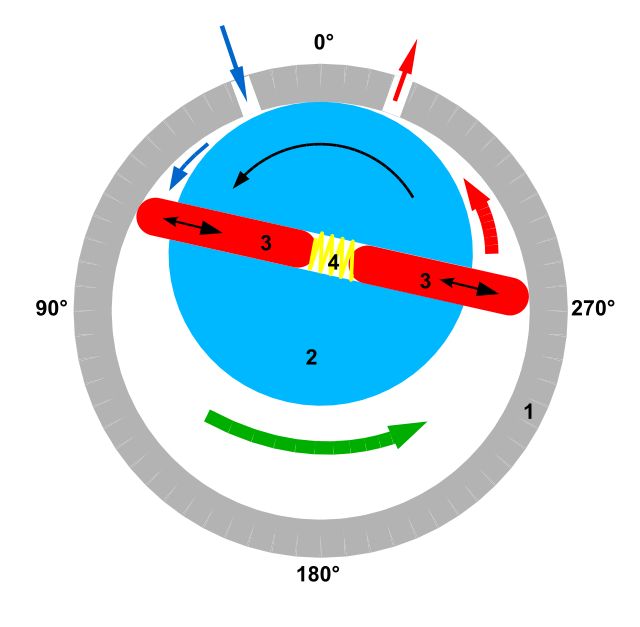
\includegraphics[scale=0.3]{Drehschieberpumpe_Schema.png}
\end{figure}


\subsection*{Turbomolekularpumpe}

Eine Turbomolkularpumpe besteht aus mehreren Stufen von fest angeorndeten Statoren. Zwischen diesen Statoren sind Rotoren, die im Bereich von $\unit[10000 - 90000]{Umd/min}$ rotieren. Das sind Geschwindigkeiten, die im Bereich der Molekülgeschwindigkeiten liegen und dadurch fügen die Rotoren den Molekülen einen zusätzlichen seitlichen Impuls hinzu. Wenn diese Komponenten groß genug ist, können die Teilchen den Rezipienten verlassen.


\subsection*{Thermovac}

Diesen Messgerät arbeitet mit der Wärmeleitfähigkeit von Gasen. Es wird eine Heizspule mit einem konstanten Strom durchflossen und auch die Temperatur soll konstant gehalten werden. Je weniger Gas vorhanden ist desto höher muss man die Spannung regeln, damit eine konstante Temperatur erreicht wird. Man kann damit bis runter auf ca $\unit[10^{-3}]{mbar}$ messen.


\subsection*{Ionivac}

Ein Ionisatios Druckmessgerät macht sich die Restelektronen in der Vakuumkammer zu nutze. Es besitzt eine Anode und eine Kathode zwischen denen eine Spannung angelegt ist. Die Elektronen werden nun von der Anode angezogen und man erhält einen von den Restelektronen abhängigen Strom.
Das Ionisations Druckmessgerät funktioniert nur bei Drücken die niedriger sind als $\unit[10^{-2}]{mbar}$, da sonst ein konstanter Strom zwischen Anode und Kathode fließen würde

\newpage


\section{Auswertung}

\subsection*{Leckrate}

\subsubsection*{Turbomolekularpumpe}

Wir bestimmen zunächst die Leckrate und betrachten dazu den Druckverlauf, als wir das Ventil dreimal kurz geschlossen haben. Für die Ausgleichsgeraden haben wir die 6 relevanten Punkte markiert:

\begin{figure}[h]
	\begin{tikzpicture}
	\begin{axis}[yticklabel style={/pgf/number format/fixed},		
	height=9cm, width=16cm,
	title={},
	legend pos= south east,
	%	     axis x line=middle, % Achse mit Pfeil und Beschriftung am Pfeil
	%	     axis y line=middle,
	xmode=normal,						    % x-Achse 
	ymode=normal,						     % y-Achse 
	xlabel= $t/s$ ,
	ylabel= $p/mbar$ ,
	grid=both, %major,
	xmin=3150,
	xmax=3750,
	ymin=0.0001,
	ymax=0.002,
	]
	\addplot[color=blue,only marks,mark=x,mark size=1, error bars/.cd,y dir=both, y explicit] table[x=t,y=p]{leckrateTurbo.txt};
	%\addlegendentry{Messwerte};
	%\addplot[color=blue,no marks,samples=1000,domain=0:7.5] {1.964*x};
	%\addlegendentry{$y = 1,964x$};
	\node[pin=0:Punkt 1] at (axis cs:3.17759E+3, 1.69000E-4 )  {};
	\node[pin=0:Punkt 2] at (axis cs:3.23609E+3, 1.95000E-3 )  {};
	\node[pin=0:Punkt 3] at (axis cs:3.40384E+3, 1.64000E-4 )  {};
	\node[pin=0:Punkt 4] at (axis cs:3.44534E+3, 1.32000E-3 )  {};
	\node[pin=0:Punkt 5] at (axis cs:3.60434E+3, 1.57000E-4 )  {};
	\node[pin=0:Punkt 6] at (axis cs:3.62984E+3, 1.16000E-3 )  {};
	\end{axis} 
	\end{tikzpicture}
\end{figure}

Die Punte sind:

\begin{center}
	$
\begin{matrix}
	Punkt	& t/s & p/mbar \\ 
	1	& 3,177\cdot 10^{3} & 1,69\cdot 10^{-4} \\ 
	2	& 3,236\cdot 10^{3} & 1,95\cdot 10^{-3} \\ 
	3	& 3,403\cdot 10^{3} & 1,64\cdot 10^{-4} \\ 
	4	& 3,445\cdot 10^{3} & 1,32\cdot 10^{-3} \\ 
	5	& 3,604\cdot 10^{3} & 1,57\cdot 10^{-4} \\ 
	6	& 3,629\cdot 10^{3} & 1,16\cdot 10^{-3}
\end{matrix} 
$	
\end{center}

Daraus können wir die Steigungen berechnen:

\begin{align*}
m_1 &= \frac{1,95 \cdot 10^{-3} - 1,69 \cdot 10^{-3}}{3,23609\cdot 10^{3} - 3,17759\cdot 10^{3}} = \unit[3,01 \cdot 10^{-5}]{mbar/s} \\
\hfil \\
m_2 &= \frac{1,32 \cdot 10^{-3} - 1,64 \cdot 10^{-3}}{3,44534\cdot 10^{3} - 3,40384\cdot 10^{3}} = \unit[2,75 \cdot 10^{-5}]{mbar/s} \\
\hfil \\
m_3 &= \frac{1,16 \cdot 10^{-3} - 1,57 \cdot 10^{-3}}{3,62984\cdot 10^{3} - 3,60434\cdot 10^{3}} = \unit[4,01 \cdot 10^{-5}]{mbar/s} 
\intertext{Der Mittelwert ist dann:}
\bar{m} &= \unit[3,25 \cdot 10^{-5}]{mbar/s} 
\end{align*}

Den Rezipienten haben haben wir vermessen und kommen auf ein Volumen von $\approx \unit[12,1]{l}$ bei einer Unsicherheit von $\approx \unit[0,4]{l}$. Die Leckrate berechnen wir dann so:

\begin{align*}
q_{pv} &= m \cdot V_{Rez} = 3,25 \cdot 10^{-5} \cdot 12,1 = \unit[3,93 \cdot 10^{-4}]{mbar \ l/s} \\
\Delta q_{pv} &= \frac{\p q_{pv}}{\p V_{Rez}} = m \cdot \Delta V_{Rez} = 3,25 \cdot 10^{-5} \cdot 0,4 = \unit[1,3 \cdot 10^{-5}]{mbar \ l/s}
\end{align*}

Damit ist unsere Leckrate $\unit[(3,93 \pm 0,13) \cdot 10^{-4}]{mbar \ l/s}$.



\subsubsection*{Drehschieberpumpe}

Nach genau dem selben Schema betrachten wie die Leckrate der Drehschieberpumpe:

\begin{figure}[h]
	\begin{tikzpicture}
	\begin{axis}[yticklabel style={/pgf/number format/fixed},		
	height=9cm, width=16cm,
	title={},
	legend pos= south east,
	%	     axis x line=middle, % Achse mit Pfeil und Beschriftung am Pfeil
	%	     axis y line=middle,
	xmode=normal,						    % x-Achse 
	ymode=normal,						     % y-Achse 
	xlabel= $t/s$ ,
	ylabel= $p/mbar$ ,
	grid=both, %major,
	xmin=4100,
	xmax=4850,
	ymin=0.0001,
	ymax=0.02,
	]
	\addplot[color=blue,only marks,mark=x,mark size=1, error bars/.cd,y dir=both, y explicit] table[x=t,y=p]{leckrateDrehschieber.txt};
	%\addlegendentry{Messwerte};
	%\addplot[color=blue,no marks,samples=1000,domain=0:7.5] {1.964*x};
	%\addlegendentry{$y = 1,964x$};
	\node[pin=0:Punkt 1] at (axis cs:4.50362E+3, 1.84000E-3 )  {};
	\node[pin=0:Punkt 2] at (axis cs:4.62812E+3, 5.35000E-3 )  {};
	\end{axis} 
	\end{tikzpicture}
\end{figure}

Die Punte sind:

\begin{center}
	$
	\begin{matrix}
	Punkt	& t/s & p/mbar \\ 
	1	& 4,50 \cdot 10^{3} & 1,84 \cdot 10^{-4} \\ 
	2	& 4,62 \cdot 10^{3} & 5,35 \cdot 10^{-3} \\ 
	\end{matrix} 
	$	
\end{center}

Daraus können wir die Steigungen berechnen:

\begin{align*}
m_1 &= \frac{5,35 \cdot 10^{-3} - 1,84 \cdot 10^{-4}}{4,62 \cdot 10^{3} - 4,50 \cdot 10^{3}} = \unit[4,305 \cdot 10^{-5}]{mbar/s} \\
\end{align*}

Wie oben ergibt sich dann die Leckrate zu:

\begin{align*}
q_{pv} &= m \cdot V_{Rez} = 4,305 \cdot 10^{-5} \cdot 12,1 = \unit[5,2 \cdot 10^{-4}]{mbar \ l/s} \\
\Delta q_{pv} &= \frac{\p q_{pv}}{\p V_{Rez}} = m \cdot \Delta V_{Rez} = 4,305 \cdot 10^{-5} \cdot 0,4 = \unit[2,08 \cdot 10^{-4}]{mbar \ l/s}
\end{align*}

Damit ist unsere Leckrate $\unit[(5,2 \pm 2,08) \cdot 10^{-4}]{mbar \ l/s}$.




\subsection*{Saugvermögen}

\subsubsection*{Drehschieberpumpe}

Um das Saugvermögen zu berechnen legen wir wieder eine Gerade durch zwei markante Punkte;

\begin{figure}[h]
	\begin{tikzpicture}
	\begin{axis}[yticklabel style={/pgf/number format/fixed},		
	height=9cm, width=16cm,
	title={},
	legend pos= south east,
	%	     axis x line=middle, % Achse mit Pfeil und Beschriftung am Pfeil
	%	     axis y line=middle,
	xmode=normal,						    % x-Achse 
	ymode=log,						     % y-Achse 
	xlabel= $t/s$ ,
	ylabel= $p/mbar$ ,
	grid=both, %major,
	xmin=0,
	xmax=200,
	ymin=0.001,
	ymax=1100,
	]
	\addplot[color=blue,only marks,mark=x,mark size=1, error bars/.cd,y dir=both, y explicit] table[x=t,y=p]{SaugrateDrehschieber.txt};
	\node[pin=0:Punkt 1] at (axis cs:8.24547E+0, 8.00000E+2 )  {};
	\node[pin=0:Punkt 2] at (axis cs:1.21497E+2, 3.40000E-1 )  {};
	\end{axis} 
	\end{tikzpicture}
\end{figure}

Die Punkte sind:

\begin{center}
	$
	\begin{matrix}
	Punkt	& t/s & p/mbar \\ 
	1	& 8,24547 \cdot 10^{0} & 8,00 \cdot 10^{2} \\ 
	2	& 1,21497 \cdot 10^{2} & 3,40 \cdot 10^{-1} \\ 

	\end{matrix} 
	$	
\end{center}


Daraus können wir die Steigungen berechnen:

\begin{align*}
|m_1| &= \left| \frac{\log\left(-3,40 \cdot 10^{-1} + 8 \cdot 10^{2}\right)}{1,21 \cdot 10^{2} - 8,24 \cdot 10^{0}} \right| = \unit[0,075]{mbar/s} \\
\end{align*}

Die Saugrate ergibt sich dann so:

\begin{align*}
S_{eff} &= m \cdot V_{Rez} = 0,075 \cdot 12,1 = \unit[0,90]{l/s} \\
\Delta S_{eff} &= \frac{\p S_{eff}}{\p V_{Rez}} = m \cdot \Delta V_{Rez} = 0,075 \cdot 0,4 = \unit[0,03]{l/s}
\end{align*}


Die Saugrate der Drehschieberpumpe ist also $\unit[(0,9 \pm 0,03)]{l/s}$


\subsubsection*{Turbomolekularpumpe}


Um das Saugvermögen zu berechnen legen wir wieder eine Gerade durch zwei markante Punkte;

\begin{figure}[h]
	\begin{tikzpicture}
	\begin{axis}[yticklabel style={/pgf/number format/fixed},		
	height=9cm, width=16cm,
	title={},
	legend pos= south east,
	%	     axis x line=middle, % Achse mit Pfeil und Beschriftung am Pfeil
	%	     axis y line=middle,
	xmode=normal,						    % x-Achse 
	ymode=log,						     % y-Achse 
	xlabel= $t/s$ ,
	ylabel= $p/mbar$ ,
	grid=both, %major,
	xmin=1910,
	xmax=1970,
	ymin=0.0001,
	ymax=0.07,
	]
	\addplot[color=blue,only marks,mark=x,mark size=1, error bars/.cd,y dir=both, y explicit] table[x=t,y=p]{SaugrateTurbo.txt};
	\node[pin=0:Punkt 1] at (axis cs:1.92277E+3, 5.55000E-2 )  {};
	\node[pin=0:Punkt 2] at (axis cs:1.93202E+3, 1.98000E-3 )  {};
	\end{axis} 
	\end{tikzpicture}
\end{figure}

Die Punte sind:

\begin{center}
	$
	\begin{matrix}
	Punkt	& t/s & p/mbar \\ 
	1	& 1,922 \cdot 10^{3} & 5,55 \cdot 10^{-2} \\ 
	2	& 1,932 \cdot 10^{3} & 1,98 \cdot 10^{-3} \\ 
	
	\end{matrix} 
	$	
\end{center}


Daraus können wir die Steigungen berechnen:

\begin{align*}
|m_1| &= \left| \frac{\log \left( -1,98 \cdot 10^{-3} + 5,55 \cdot 10^{-2} \right)}{1,932 \cdot 10^{3} - 1,922 \cdot 10^{3}} \right| = \unit[0,127]{mbar/s} \\
\end{align*}

Die Saugrate ergibt sich dann so:

\begin{align*}
S_{eff} &= m \cdot V_{Rez} = 0,127 \cdot 12,1 = \unit[1,5]{l/s} \\
\Delta S_{eff} &= \frac{\p S_{eff}}{\p V_{Rez}} = m \cdot \Delta V_{Rez} = 0,127 \cdot 0,4 = \unit[0,05]{l/s}
\end{align*}


Die Saugrate der Turbomolekularpumpe ist also $\unit[(1,5 \pm 0,05)]{l/s}$



\subsubsection*{Theoretisches Saugvermögen der Turbopumpe}

Um das theoretische Saugvermögen zu bestimmen, müssen wir die Rohrdurchmesser und Längen der einzelnen Abschnitte berücksichtigen. Zudem wissen wir aus dem Datenblatt, das die maximale Pumpleistung der Turbopump bei $\approx \unit[55]{l/s}$ liegt. Daraus erhalten wir nun:

\hfill \\

\begin{tabular}{c|c|c|c|c|c}
	& Länge / cm & Durchmesser / cm & Klausius & Leitwert / l/s & 1/Leitwert / s/l \\
	\hline 
	&      &      &      &      &  \\
	Schiebeventil 1 & 1,8  & 3,2  & 0,27084054 & 60,7674301 & 0,01645618 \\
	Schiebeventil 2 & 1,8  & 3,2  & 0,27084054 & 60,7674301 & 0,01645618 \\
	Schiebeventil 3 & 2,4  & 2,4  & 0,38571429 & 27,3821773 & 0,03652011 \\
	Winkelstück & 15,394 & 3,6  & 0,70553244 & 26,3543786 & 0,03794436 \\
	Flansch & 8,7  & 2,3  & 0,68101282 & 11,7381407 & 0,08519237 \\
	Pumpe &      &      &      & 55   & 0,01818182 \\
\end{tabular}

\hfill \\

Die Leitwerte werden nach folgender Formel berechnet:

\begin{align*}
c &= K'' \cdot 3,81 \cdot \sqrt{\frac{T}{M}} \cdot \frac{D^3}{L}
\intertext{Der Klausiusfaktor $K''$ lässt sich dann so bestimmen:}
K'' &= \frac{15 \cdot \frac{L}{D} + 12 \cdot \left( \frac{L}{D} \right)^2}{20 + 38 \cdot \frac{L}{D} + 12 \cdot \left( \frac{L}{D} \right)^2}
\intertext{Zudem wir die Länge des gekrümmten Rohrs wie folgt umgerechnet:}
l &= l_{ax} + 1,33 \cdot \frac{90}{180} \cdot D
\intertext{Für das theoretische Saugvermögen ergibt sich dann:}
S_{theo} &= \frac{1}{\sum \left( 1/Leitwert \right)} = \unit[4,755]{l/s}
\end{align*}


Das theoretische Saugvermögen liegt also um knapp den Faktor 4 über dem gemessenen.


\newpage

\subsubsection*{Leckraten bei laufenden Pumpen}


Die Leckraten können wir nach folgender Formel bestimmen:

\[C = \frac{P_e \cdot S_{eff}}{P_a}\]

\paragraph*{Turbopumpe} 

\hfill \\

Für die Turbopumpe ergibt sich dann:

\begin{align*}
C &= \frac{1,5 \cdot 1,69 \cdot 10^{-4}}{1013} = \unit[2,5 \cdot 10^{-7}]{l/s}
\end{align*}


\paragraph*{Drehschieberpumpe} 

\hfill \\

Für die Drehschieberpumpe ergibt sich dann:

\begin{align*}
C &= \frac{0,9 \cdot 8 \cdot 10^{-3}}{1013} = \unit[7,1 \cdot 10^{-6}]{l/s}
\end{align*}












\end{document}